\section{Software Performance} \label{chapter3:software-performance}

% The previous section showed that modular programming limits performance scalability of execution.


Moore's law \cite{Moore1965} which forecasts the density of transistors per processing unit, was wrongly interpreted to promise the exponential evolution in the sequential performance of the processing unit, and the assurance for the software industry of always faster hardware.
But as transistors attained a critical size, the reduction in power required by transistor predicted by the Dennard's MOSFET scaling \cite{Dennard2007} stopped\ftnt{https://cartesianproduct.wordpress.com/2013/04/15/the-end-of-dennard-scaling/}.
The ever growing number of transistor predicted by Moore's law are arranged in parallel architecture to continue increasing the performance of processing units.
Parallel programming became the only solution for scalable performance, at the expense of development effort.

This section presents the parallel programming solutions and their limitations in accessibility, and then the improvements to overcome these limitations.

\subsection{Parallel Programming} \label{chapter3:software-performance:parallel-programming}


Concurrent programming is based on the causal ordering of execution.
The ordering of operations is local within a synchronous execution, while the concurrent executions are causally ordered.
It leads to parallel execution with some coordinations such as synchronization, immutability or isolation.
As Lamport showed \cite{Lamport1978}, and Reed related later \cite{Reed2012}, This causal order is sufficient to execute correctly a system in parallel, such as in distributed system.

\begin{center}
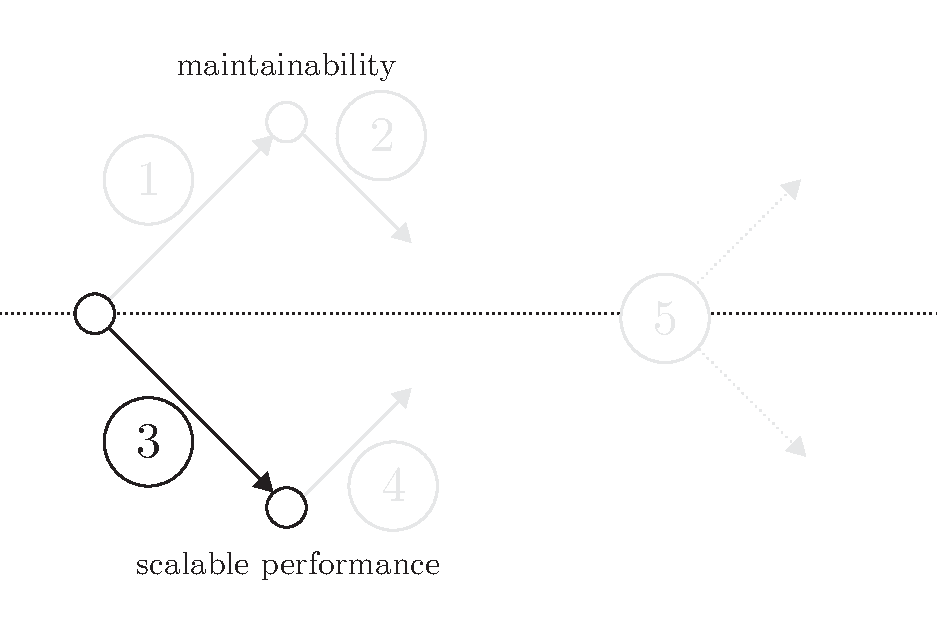
\includegraphics[width=0.6\textwidth]{../ressources/state-of-the-art-3.pdf}
\end{center}

This section presents first hand the theoretical and programming model based on asynchronous communication and isolated execution for parallel programming, as illustrated on the schema above.
It then continues with stream processing programming model. 
And finally,it concludes on the limitations of parallel programming regarding accessibility. 






% All these early work adopted concurrent composition by default, instead of sequential composition, to adapt to the very concurrent nature of real parallel machines.
% However, sequential programming is still the default.
% Concurrent composition is yet still to be widely accepted, as stated by Reed \cite{Reed2012}.
% \comment{TODO rewrite this paragraph}
% \sout{
% % The Actor Model uses asynchronous communications, while $\pi$-calculus uses synchronous communications.
% % Synchronous communications are deterministic.
% % The message sent needs to be received to continue the execution on both ends.
% Because of the synchronous communication used by $\pi$-calculus, the concurrent executions and the communications are both deterministic.
% Therefore, the result of the concurrent system is assured to be deterministic.
% The correctness of the execution of deterministic systems is guaranteed.
% % Determinism is a wanted property to assure the correctness of the execution.
% }

% \sout{
% On the other hand, the asynchronous communications used by Actors are non-deterministic.
% The message sent can take an infinite time to be received.
% Therefore, the result of the concurrent system is not assured to be deterministic.}

% The communication in reality are subject to various faults and attacks \cite{Lamport1982} and too slow compared to execution to be synchronous.

% % And the wait required by synchronous communications negatively impact performances of the system because of the difference of latency between communication, and execution.
% The Actor model was explicitly designed to take these physical limitations in account \cite{Hewitt1977a}.
% The non-determinism in the asynchronous communications is hidden by the organization of the system.
% The total ordering of execution possible with synchronous communication is too strong a requirement for correctness.

% % The non-determinism in the asynchronous communications is hidden by the organization of the system.
% The ordering of execution is only local to an \comment{entity}, while between \comment{entities}, execution is causally ordered.
% The execution will either terminate correctly, or not terminate at all because of a failure in the communications.




% Asynchronous communications are less expressive than synchronous ones \cite{PALAMIDESSI2003}.

% Pi-calculus is a synchronous paradigm which contains an asynchronous fragment.\cite{PALAMIDESSI2003}
% (Boudol, G. (1992). Asynchrony and the π-calculus (note). Rapport de Recherche  1702, INRIA, Sophia-Antipolis,
% Honda, K. and Tokoro, M. (1991).  An object calculus for asynchronous communication. In America, P., editor, Proceedings of the European Conference on Object-Oriented Programming (ECOOP), volume 512 of Lecture Notes in Computer Science, pages 133–147. Springer-Verlag)


% The asynchronous pi-calculus defined by Honda and Tokoro in 1991 led to Pict, a programming language\cite{Pierce2000}.




% There was firstly theories, and models for concurrent computation.
% The main problem was determinism.
% In a sequential machine, the non-determinism of the physical world is hidden by the sequentiality of the machine.
% However, in concurrent computation, the order of communication cannot be assured the way the order of statements is assured in a sequential machine.
% We observe local non-determinism.
% However, to conserve an apparent determinism, causal ordering is sufficient.


\subsubsection{Asynchronous and Isolated Process Parallelism}

The Flynn's taxonomy \cite{Flynn1972} is the most commonly used to categorize parallel execution.
It separates the flow of instructions, and the flow of data ; each being unique, or multiple.
All the current parallel programming model currently belong to the category Multiple Instruction Multiple Data (MIMD), which is further divided into Single Program Multiple Data (SPMD) \cite{Auguin1983,Darema1988,Darema2001} and Multiple Program Multiple Data (MPMD) \cite{Chang1997,Chan2004}.
MIMD implies several threads of execution processing several stream of data.
% The difference between SPMD and MPMD holds on the distinction of instruction pool between the threads of execution.
% SPMD implies to replicate the same program on all the processing units, while MPMD implies to define different programs for every processing units.

% \begin{figure}
% \begin{center}
% 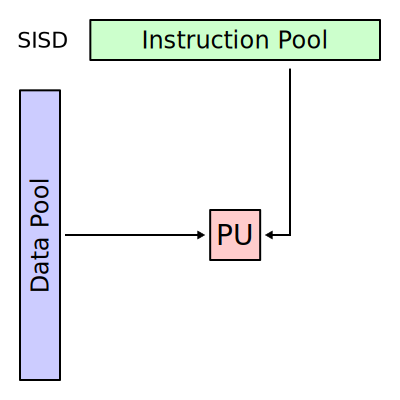
\includegraphics[width=0.2\textwidth]{../ressources/SISD.svg}
% 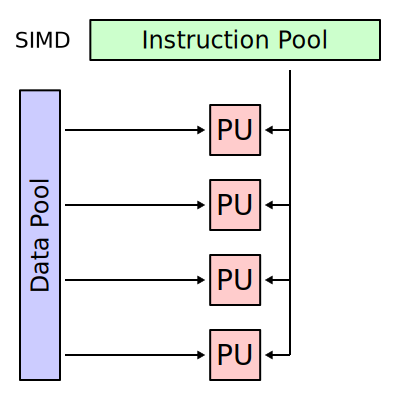
\includegraphics[width=0.2\textwidth]{../ressources/SIMD.svg}
% 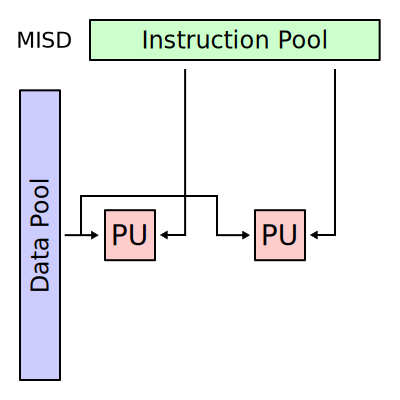
\includegraphics[width=0.2\textwidth]{../ressources/MISD.svg}
% 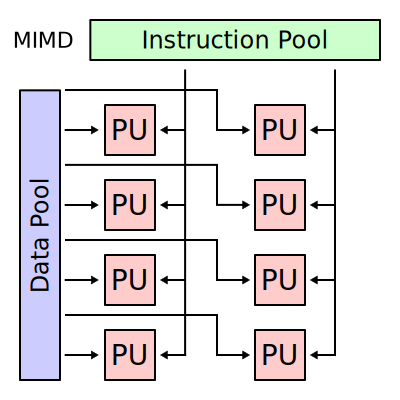
\includegraphics[width=0.2\textwidth]{../ressources/MIMD.svg}\\
% by I, Cburnett. Licensed under CC BY-SA 3.0 via Commons
% \url{https://commons.wikimedia.org/wiki/File:SISD.svg#/media/File:SISD.svg}
% \url{https://commons.wikimedia.org/wiki/File:SIMD.svg#/media/File:SIMD.svg}
% \url{https://commons.wikimedia.org/wiki/File:MISD.svg#/media/File:MISD.svg}
% \url{https://commons.wikimedia.org/wiki/File:MIMD.svg#/media/File:MIMD.svg}
% \end{center}
% \nt{TODO convert these svg to pdf}
% \caption{Flynn's taxonomy of parallelism}
% \end{figure}

\nt{schemas SPMD / MPMD}

The difference between SPMD and MPMD is in the representation of the execution in implementation.
SPMD organizes the implementation as a single execution replicated on many processing units.
While MPMD organizes explicitly the different threads of execution in the implementation.
Examples of SPMD programming languages are
Split-C \cite{Culler},
CRL \cite{Johnson1995} and
Composite C++ \cite{K.ManiChandy2005}.
%
Examples of MPMD programming languages are
Mentat \cite{Grimshaw1991},
Fortran M \cite{Foster1995b} and
Nexus \cite{Foster1996}.
SPMD is close to the model presenting parallel improvements over modular programming presented in section \ref{chapter3:software-design:programming-models}.
While MPMD is closer to the programming models based on isolated process presented in the remaining of this section.
The coordinations between these threads of execution were done by message passing, using PVM \cite{Sunderam1994}, MPI \cite{Snir1996,Walker1996}, SOAP, or the more recent REST protocols.



\paragraph{Theoretical Models}


The communication in reality are subject to various faults and attacks \cite{Lamport1982} and too slow compared to execution to be synchronous.
The Actor model is one of the first programming model to be explicitly designed to take these physical limitations in account \cite{Hewitt1977a}.
It allows to express the computation as a set of communicating actors \cite{Hewitt1973a, Hewitt1977, Clinger1981}.
In reaction to a received message, an actor can create other actors, send messages, and choose how to respond to the next message.
All actors are executed concurrently, and communicate asynchronously.
An asynchronous communication implies that the sender continues its execution immediately after sending the message, before receiving the result of the initiated communication.

In the Actor Model, everything is an actor, even the simplest types like numbers.
This level of granularity is unachievable in practice due to overhead from the asynchronous communications.
Most implementations adopt a granularity on the process or function level.

Coroutines are autonomous programs which communicate with adjacent modules as if they were input and output subroutines \cite{Conway1963}.
It is the first definition of a pipeline to implement multi-pass algorithms.
Similar works include the Communicating Sequential Processes (CSP) \cite{Hoare1978, Brookes1984}, and the Kahn Networks \cite{Kahn1974, Kahn1976}.

% \sout{The first models of computation, like the Turing machine and lambda-calculus, were sequential and based on a global memory state.
% A formalism was missing to represent concurrent computations.
% This section presents the most important works on formalisms for parallel computation.
% They tackled the problems of determinacy, state synchronization and correctness of execution in a formalism based on a network of concurrent processes, asynchronously communicating via messages.
% This section first presents the works on the programming models based on this formalism.
% Then it presents the huge improvements we recently witnessed in the field of distributed stream processing due to the need of performance from the web to process large stream of requests,}

% The mathematical models are a ground for all following work on concurrent programming, we briefly explain them in the next paragraphs.
% There are two main formal models for concurrent computations.
% The Actor Model of C. Hewitt and the Pi-calculus of R. Milner.
% Based on these definitions, we explain the importance of determinism for correctness, and the reasons that made asynchronous message-passing prevail.

% TODO illustration of cells, and draw an analogy between cells and actor model.
% Or something the actor models is based upon.


% The Actor model allows to express the computation as a set of communicating actors \cite{Hewitt1973a, Hewitt1977, Clinger1981}.
% In reaction to a received message, an actor can create other actors, send messages, and choose how to respond to the next message.
% All actors are executed concurrently, and communicate asynchronously.
% The Actor model uses an asynchronous message-passing communication paradigm.
% The communication between two actors, the sender and the receiver, is a stream of discrete messages.
% The sender names the receiver actor when sending messages to be the recipient of these messages.
% An asynchronous communication implies that the sender continues its execution immediately after sending the message, before receiving the result of the initiated communication.

% The Actor model was presented as a highly parallel programming model, but intended for Artificial Intelligence purposes.
% Its success spread way out of this scope, and it became a general reference and influence.
% For example, the Scala programming language features an actor approach to concurrency.

% More recent work of C. Hewitt on Actors is about ... \nt{TODO} \cite{Hewitt2007,Hewitt2007a}.


% R. Milner presented a process calculus to describe concurrent computation : the Calculus of Communicating Systems (CCS) \cite{Milner1975, Milner1980}.
% It is an algebraic notation to express identified processes communicating through synchronous labeled channels.
% % In CCS, process compose concurrently, communications are synchronous, and the topology is static.
% The $\pi$-calculus improved upon this earlier work to allow processes to be communicated as values, hence to become mobile \cite{Engberg1986,Milner1992a,Milner1992}.
% Therefore, similarly to Actors, in Pi-calculus processes can dynamically modify the topology.
% However, contrary to the Actor model, communications in Pi-calculus are based on simultaneous execution of complementary actions, they are synchronous.








% The theory advocates asynchronous message-passing, but it doesn't precise the granularity of the communicating entities.
% In the Actor Model, everything is an actor, even the simplest types, like numbers, similarly in OOP, everything is an object.
% In practice, this level of granularity is unachievable due to overhead from the asynchronous communications.
% Most implementations adopt a granularity on the process or function level.

% % concurrent programming
% The first concept using message passing was the coroutine.
% % It influenced many following works.
% Conway defines coroutines as an autonomous program which communicate with adjacent modules as if they were input and output subroutines \cite{Conway1963}.
% It is the first definition of a pipeline to implement multi-pass algorithms.
% Similar works include the Communicating Sequential Processes (CSP) \cite{Hoare1978, Brookes1984}, and the Kahn Networks \cite{Kahn1974, Kahn1976}.

% Hoare presented the Communicating Sequential Processes (CSP) \cite{Hoare1978, Brookes1984}.
% These processes are executed concurrently, and communicates events via named channels.
% The evolutions of this model were influenced by, and influenced the work of Milner that led to $\pi$-calculus.

% Similarly, Kahn developed the Kahn Networks \cite{Kahn1974, Kahn1976}, following the work of Conway on coroutines.
% They are explicitly parallel coroutines separated by bounded FIFO streams for communication.



% The shared-nothing architecture \cite{Stonebraker1986}.


\paragraph{Programming Languages}

The theoretical models presented above are implemented in industrial languages such as Akka Scala and Erlang.

Scala is an attempt at unifying the object model, and functional programming \cite{Odersky2004}.
% It proposes an actor approach in its design.
Akka\ftnt{http://akka.io/} is a framework based on Scala, following the Actor model to build higly scalable and resilient applications.
Play\ftnt{https://www.playframework.com/} is a web framework based on top of Akka.

Erlang borrow the Actor model as well.
It is a functional concurrent language designed by Ericsson to operate telecommunication devices \cite{JoeArmstrong,Nelson2004} % Nelson2004 is not very good, find another better citation.

\nt{review this paragraph and the transition to the next section}
The field of concurrent programming is so vast it is impossible to relate here every programming languages.
The previous examples are only the best known.
The next focus focuses on streaming real-time applications.

% \comment{transition on lazy evaluation equivalence to stream. lazy evaluation + side effects + concurrency = streams}

\subsubsection{Stream Processing Systems}

All the solutions previously presented are designed to build general distributed systems.
In the context of the web, a real-time application must process high volumes streams of requests within a certain time.
Because these systems are key to business, their reliability and latency are of critical importance.
Otherwise, input data may be lost or output data may lose their value.
These requirements are challenging to meet in the design of such system.

% \textit{
% From a language designer's point of view, real-time
% programs have these characteristics:
% \begin{enumerate}
% \item A real-time program interacts with an environ-
% ment in which many things happen simultaneously at
% high speeds.
% \item A real-time program must respond to a variety
% of nondeterministic requests from its environment. The
% program cannot predict the order in which these requests
% will be made but must respond to them within certain
% time limits. Otherwise, input data may be lost or output
% data may lose their significance.
% \item A real-time program controls a computer with a
% fixed configuration of processors and peripherals and
% performs (in most cases) a fLxed number of concurrent
% tasks in its environment.
% \item A real-time program never terminates but contin-
% ues to serve its environment as long as the computer
% works. (The occasional need to stop a real-time program,
% say at the end of an experiment, can be handled by ad
% hoc mechanisms, such as turning the machine off or
% loading another program into it.)
% \end{enumerate}
% }




\paragraph{Data-stream Management Systems}

% The processing of large volume of data was historically handled by Database management systems.
% These systems naturally evolved to manage data-streams as well.

Database Management Systems (DBMS) historically processed large volume of data, and they naturally evolved into Data-stream Management System (DSMS) to processed data streams as well.
Because of this evolution, they are in rupture with imperative languages presented until now, and borrow the syntax from SQL.

DSMS concurrently run SQL-like requests on continuous data streams.
The computation of these requests spread over a distributed architecture.
Among the early works, we can cite
NiagaraCQ \cite{Chen2000,Naughton2001},
Aurora \cite{Abadi2003,Abadi2003a,Balakrishnan2004} which evolved into
Borealis \cite{Abadi2005},
AQuery \cite{Lerner2003},
STREAM \cite{Arasu2003,Arasu2005} and
TelegraphCQ \cite{Krishnamurthy2003,Chandrasekaran2003}.
More recently, we can cite
DryadLINQ \cite{Isard2007,Yu2009},
Apache Hive \cite{Thusoo2009}\ftnt{https://hive.apache.org/},
Timestream \cite{Qian2013} and
Shark \cite{Xin2013}.


  % + Grape / Timestream - distributed SQL (roughly)
  % + CQL
  % +> STREAM (uses CQL)
  % + StreaQuel
  % +> TelegraphCQ
  % + AQuery

  % + 

% SQL-like
%   AQuery \cite{Lerner2003}
%   STREAM (uses CQL) \cite{Arasu2003,Arasu2005}
%   TelegraphCQ (uses StreaQuel) \cite{Krishnamurthy2003,Chandrasekaran2003}
%   Grape / Timestream - distributed SQL (roughly) \cite{Qian2013}
%   Shark        Stateless dataflow \cite{Xin2013}

%   DryadLINQ    Stateless dataflow \cite{Isard2007,Yu2009}

% \subsubsection{Batched dataflow}

% Map/Reduce
%   MapReduce    Stateless dataflow \cite{Dean2008}
%   Hadoop       Stateless dataflow 
%   Incoop       Incremental dataflow \cite{Bhatotia2011}

% Functional
%   Comet        Batched dataflow \cite{He2010}
%   D-Streams    Batched dataflow \cite{Zaharia2012}
%   Spark        Stateless dataflow \cite{Zaharia,Zaharia2010}
%   Nectar       Incremental dataflow \cite{Gunda2010}





% Imperative Stream Processing
%   Piccolo                                  Parallel in-memory \cite{Power2010}
%   CIEL                                    Stateless dataflow \cite{Murray2011}
%   Statdeful Dataflow Graph (SDG)          Stateful dataflow  \cite{Fernandez2014a}


\paragraph{Pipeline Architecture}

As presented in the previous section, streaming and lazy-evaluation composition both allow a loosely coupled yet efficient composition.
The pipeline architecture takes advantage of this, and composes the parallel execution in a stream, the output of one feeding the input of the next.

SEDA is a precursor in the design of pipeline-based architecture for real-time web applications \cite{Welsh2001}.
It organizes an application as a network of event-driven stages connected by explicit queues.
The event-driven paradigm is similar to previous web servers implementations like Ninja and Flash \cite{Gribble2001,Pai1999}.
SEDA improves with the pipeline organization in stages.

Several projects followed and adapted the principles in this work.
StreaMIT is a language to help the programming of large streaming application \cite{Thies2002}.
Storm \cite{Toshniwal2014} is designed by and used at Twitter to process the heavy streams of tweets.
% It is only one example of industrial practical application, among many others.
Among other works, in the industry, there are
CBP \cite{Logothetis2010} and
S4 \cite{Neumeyer2010}, that were designed at Yahoo,
Millwheel \cite{Akidau2013} designed at Google and
Naiad \cite{Murray2013} designed at Microsoft.

In the litterature, there are
Spidle \cite{Consel2003},
Pig Latin \cite{Olston2008},
Piccolo \cite{Power2010},
Comet \cite{He2010},
Nectar \cite{Gunda2010},
SEEP \cite{Migliavacca2010} and
SDG \cite{Fernandez2014a}

% Similarly to the programming models presented in section \ref{chpater3:concurrent-programming:programming-languages} these frameworks are elitist and not accessible to a large community of developers.
% Indeed, the pipeline architecture presents a distributed storage, which is hardly compatible with the best practices.
% It impacts maintainability.
% For this reason, there are some works on reconciling the concurrent programming models with the modular programming model favoring maintainability.

% + Spidle: A DSL approach to specifying streaming applications dataflow like 


% + Blazes: Coordination analysis for distributed programs \cite{Alvaro2014}



%   (From the paper : Making state explicit for imperative big data processing)
%   + MapReduce       map/reduce   |   Stateless dataflow
%   + DryadLINQ       functional   |   Stateless dataflow
%   + Spark           functional   |   Stateless dataflow
%   + CIEL            imperative   |   Stateless dataflow
%   + Hadoop          map/reduce   |   Stateless dataflow
%   + Incoop          map/reduce   |   Incremental dataflow
%   + Nectar          functional   |   Incremental dataflow
%   + CBP             dataflow     |   Incremental dataflow
%   + Comet           functional   |   Batched dataflow
%   + D-Streams       functional   |   Batched dataflow
%   + Naiad           Dataflow     |   Batched dataflow
%   + Storm, S4       dataflow     |   Continuous dataflow
%   + SEEP            dataflow     |   Continuous dataflow
%   + Piccolo         imperative   |   Parallel in-memory
%   + SDG             imperative   |   Stateful dataflow

%   + pig https://pig.apache.org/
  
% Dataflow
%   CBP          Incremental dataflow \cite{Logothetis2010}
%   S4           Continuous dataflow \cite{Neumeyer2010}
%   Storm        Continuous dataflow \cite{Toshniwal2014}
%   Millwheel    Continuous dataflow \cite{Akidau2013}
%   SEEP         Continuous dataflow \cite{Fernandez2013}
%   Naiad        Batched dataflow \cite{Murray2013}





\comment{Transition on the limitations of software parallelism}

\subsubsection{Elitism of Parallel Programming}

In these parallel programming models describing a network of isolated execution, the topology of the network is statically defined. 
The dynamical modification of the topology is impossible.
It is not possible to dynamically manipulate execution containers, like it is possible to manipulate functions.
Therefore, higher-level programming is impossible, so modular programming is limited.

Moreover, the decomposition of the execution and memory required is difficult for most developers to manage correctly.
\nt{TODO make sure this idea is correctly developed throughout this chapter : parallel programming implies to keep a double mental representation.}
It implies to keep two mental representation of the implementation.
One for the modularity, and one for the decomposition of execution.
Parallel programming remains hard, and is accessible only to an elite of developers.

The next section presents different improvements to make parallel programming more accessible to common developers.





\begin{table}
\small
\begin{tabu} to \linewidth {@{} *1{X[c]} | *2{X[c]} | *1{X[c]} | *2{X[c]} @{}}
%
\toprule
\multicolumn{3}{c}{}  & \multicolumn{1}{|c|}{Concurrency} & \multicolumn{2}{|c}{Parallelism} \\
& Model & Examples    & \multicolumn{1}{|c|}{Synchronization} & Immutability & Isolation \\
\midrule
% ✖ ⨯ ✔                                                                     SYN  IMU  ISO
\multirow{4}{*}{\begin{sideways}\parbox{2.2cm}{Parallel Programming}\end{sideways}} & %
  \multirow{2}{*}{Actor Model}          & Scala, Akka, Play                 & \X & \V & \V \\
&                                       & Erlang                            & \X & \V & \V \\
& \multirow{2}{*}{Stream Processing}    & DSMS (Timestream)                 & \X & \V & \V \\
&                                       & Pipeline (SEDA)                   & \X & \V & \V \\
\bottomrule
\end{tabu}
\caption{Synthesis of the state of the art in parallel programming}
\end{table}














\subsection{Maintainability Improvements} \label{chapter3:software-performance:maintainability}

\comment{Introduction}

As the limitations above state, the difficulties in parallel programming are the absence of higher-level programming, and the decomposition of execution and memory required for parallelism.
This section presents the improvements on accessibility in parallel programing, as illustrated in the schema below.

\begin{center}
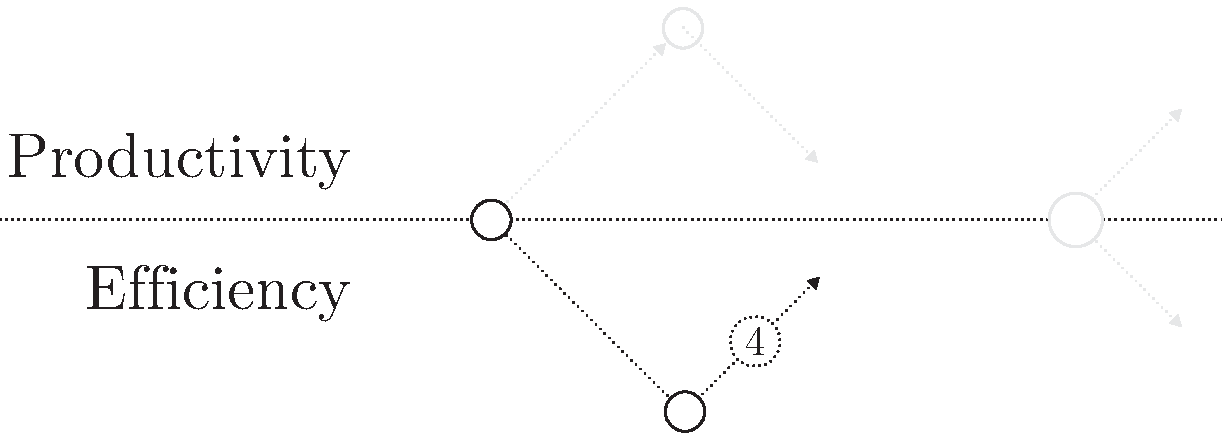
\includegraphics[width=0.6\textwidth]{../ressources/state-of-the-art-4.pdf}
\end{center}

These improvements holds on execution or memory.
This section presents firstly the improvements to ease the decomposition of execution through design patterns and different granularities.
It then presents the improvements to helps development in face of the required memory isolation for distribution.
It then transitions to the lack of improvements for higher-order programming in parallel programing.

\subsubsection{Execution Organization}

All of the parallel programming models presented above decompose the execution into isolated parallel executions, like actors.
This decomposition is difficult as it implies to manage both the parallel decomposition of execution and the modular decomposition of implementation.
Most developers are unable to manage efficiently the two decompositions.
The next paragraphs presents some solutions to mitigate this duality.
\nt{TODO weak argumentation}

\paragraph{Design Patterns}

To reduce the difficulties of the decomposition of the execution into actors, algorithmic skeletons propose predefined patterns that fit certain type of problems \cite{Cole1988, Dean2008, McCool2010, Gonzalez-Velez2010}.
A developer implements the problem as a specific case of a skeleton.
It simplifies the communications, so that the developer can focus on its problem independently of message passing required by the distribution of execution.

% \nt{Link with DSMS}
% As there is similtudes between SQL-like languages, functional structures, and algorithmic skeletons, the latter can be seen as a tentative to merge the more descriptional features of the former into imperative programming.
% Indeed, among the Algorithmic skeletons, we can cite Map / reduce, which are functional structures, but are somehow equivalent to the select and aggregate functions of SQL.
% The pipeline architecture for data stream processing presented in section \ref{chapter3:software-efficiency:dataflow-pipeline} can be considered as algorithmic skeletons.

% However, they introduce limitations and difficulties, as the developer must fit its problem into the skeletons.
% One of this difficulties, it that a common memory is impossible to use.
% Developers needs to think in terms of message passing instead of a global memory, which, as we saw in previous section, is incompatible with best practices.

% Introducing 'Bones': a parallelizing source-to-source compiler based on algorithmic skeletons \cite{Nugteren2012}

\paragraph{Granularity}

The Service Oriented Architectures (SOA), and more recently Microservice\cite{Namiot2014,Fernandez-Villamor2010,Fowler2014,Namiot2014} allow developers to express an application as an assembly of services connected to each others.
Some examples of frameworks are OSGi\ftnt{https://www.osgi.org/developer/specifications/}, EJB\ftnt{http://www.oracle.com/technetwork/java/javaee/ejb/index.html}, Spring\ftnt{http://projects.spring.io/spring-framework/}, and Seneca\ftnt{http://senecajs.org/}
It intends to adjust the granularity of execution decomposition to help developers to fit the two organizations, the modular organization and the parallel execution organization \cite{Adam2008}.

% In modular programming a module protects the rest of the implementation from the consequences of the design choice its encapsulate, while a service encapsulate a specific task, with possible consequences on the adjacent services.

% In a fine enough granularity of service, each service becomes so simple, it can limits the consequences of its modification.

\paragraph{Dynamic Distribution}

An interesting work following SEDA, is Leda \cite{Salmito2013,Salmito2014}.It follows the PCAM design methodology \cite{Foster1995} to propose a model where the stages of the pipeline are defined only by their role in the application.
% Partition $\to$ Communicate $\to$ Agglomerate $\to$ Map.
The actual execution distribution in stages is defined automatically, only after the development, during deployment.
This automation blurs the distinction between the parallel organization of execution, and the modular organization of implementation.
It manages the execution organizations to helps the developer focus on the modular organization.

\paragraph{}

These works helps developers to decompose and distribute the execution of a parallel application.
However, they still propose a distributed memory model.
It doesn't allow higher-level programming, and it requires developers to distribute the state of the application, and assure its isolation.
For these two reason it is difficult to manage.
The next paragraph presents works to improve on the distribution of memory.

% Though, they are still independent, so higher-level programming is impossible.

\subsubsection{Memory Abstraction}

Parallelization of the execution eventually requires the distribution of the memory.
The Partitioned Global Address Space (PGAS) provides the developers with a uniform memory access on a distributed architecture.
It attempts to combine the advantage of SPMD programming style for distributed memory systems, with the data referencing semantics of shared memory systems.
Each computing node executes the same program, and provide its local memory to be shared with all the other nodes.
The PGAS programming model assure the remote accesses and synchronization of memory across nodes, and enforces locality of reference, to reduce the communication overhead.
Examples of implementation of the PGAS model are 
Chapel\cite{Chamberlain2007},
X10 \cite{Charles2005}.
Unified Parallel C \cite{El-Ghazawi2006},
CoArray Fortran \cite{Numrich1998} and
OpenSHMEM \cite{Chapman2010}.

% These programming models are promising.
% However, they focus rather on scientific application with intensive computing such as matrix multiplication, and leave out streaming applications, such as web services.

\paragraph{}

% \nt{TODO PGAS are similar to the programming models presented in the previous section (synchronization).}

The PGAS programming model is similar to the Multi-Threading Programming model presented in section \ref{chapter3:software-maintainability:performance:concurrent-programming}. 
However, it is more focused on performance than modularity.
It focuses on scientific applications with intensive computing such as matrices multiplication.
%, and leave out streaming applications, such as web services.


\subsubsection{Lack of Higher-Order Programming}

% Moreover, 
The programming models of this section lack higher order programming.
% Moreover, in these solutions, higher-order programming is impossible.
As showed earlier in section \ref{chapter3:software-design:programming-models:functional-programming}, higher-order programming is important for modular design and maintainability of the implementation.
In this regards, parallel programming seems currently incompatible with modular programming.
The next section presents the proposition of this thesis to bring parallel programming to a higher-order programming language.
% By keeping the modular programming model, the compilation approach allows higher-level programming.

% \paragraph{Transistion : these methods doesn't allow higher-order programming, which is required for good modularity. WHY ?}

% \nt{TODO link with 3.1}


\begin{table}
\small
\begin{tabu} to \linewidth {@{} *1{X[c]} | *2{X[c]} | *3{X[c]} @{}}
%
\toprule
\multicolumn{3}{c}{} & \multicolumn{3}{|c}{Modularity} \\
& Model & Examples     & Higher-Order Programming & Closures & Lazy Evaluation / Streams \\
\midrule
% ✖ ⨯ ✔                                                                       HOP  CLS  LZY  SYN  IMU  ISO
\multirow{4}{*}{\begin{sideways}\parbox{2.2cm}{Maintainability Improvements}\end{sideways}} & %
  Algorithmic Skeletons                 & Map Reduce ...                    & \X & \X & \V \\
& SOA, Microservices                    & EJB, Spring, Seneca               & \X & \X & \V \\
& Dynamic Distribution                  & LEDA                              & \X & \X & \V \\
& PGAS                                  & Chapel, X10 ...                   & \X & \X & \X \\
\bottomrule
\end{tabu}
\caption{Synthesis of the state of the art in maintainability improvements for parallel programming}
\end{table}













\endinput

\subsection{Concurrency Theory} \label{chapter3:parallel-execution:concurrency-theory}

The mathematical models are a ground for all following work on concurrent programming, we briefly explain them in the next paragraphs.
There are two main formal models for concurrent computations.
The Actor Model of C. Hewitt and the Pi-calculus of R. Milner.
Based on these definitions, we explain the importance of determinism for correctness, and the reasons that made asynchronous message-passing prevail.

% TODO illustration of cells, and draw an analogy between cells and actor model.
% Or something the actor models is based upon.

\subsubsection{Models}

\paragraph{Actor Model}

The Actor model allows to express the computation as a set of communicating actors \cite{Hewitt1973a, Hewitt1977, Clinger1981}.
In reaction to a received message, an actor can create other actors, send messages, and choose how to respond to the next message.
All actors are executed concurrently, and communicate asynchronously.
% The Actor model uses an asynchronous message-passing communication paradigm.
% The communication between two actors, the sender and the receiver, is a stream of discrete messages.
% The sender names the receiver actor when sending messages to be the recipient of these messages.
An asynchronous communication implies that the sender continues its execution immediately after sending the message, before receiving the result of the initiated communication.

The Actor model was presented as a highly parallel programming model, but intended for Artificial Intelligence purposes.
Its success spread way out of this scope, and it became a general reference and influence.
% For example, the Scala programming language features an actor approach to concurrency.

% More recent work of C. Hewitt on Actors is about ... \nt{TODO} \cite{Hewitt2007,Hewitt2007a}.

\paragraph{$\pi$-calculus}

R. Milner presented a process calculus to describe concurrent computation : the Calculus of Communicating Systems (CCS) \cite{Milner1975, Milner1980}.
It is an algebraic notation to express identified processes communicating through synchronous labeled channels.
% In CCS, process compose concurrently, communications are synchronous, and the topology is static.
The $\pi$-calculus improved upon this earlier work to allow processes to be communicated as values, hence to become mobile \cite{Engberg1986,Milner1992a,Milner1992}.
Therefore, similarly to Actors, in Pi-calculus processes can dynamically modify the topology.
However, contrary to the Actor model, communications in Pi-calculus are based on simultaneous execution of complementary actions, they are synchronous.


% Actors can create actors, pi-caclulys processes can replicate, and send processes through channel.
% Processes create a new processes on each instruction to continue the execution.!g systolic arrays

% Pi-calculus resembles to the actor model, but its algebraic nature led to a critical difference with the latter.
% Indeed, processes in the Pi-calculus communicate indirectly, through labeled ports, whereas actors communicate directly by naming the recipient actors.
% This difference allows multiple processes to listen in turns to the same channel, whereas the recipient of a message cannot change.

% I think this difference lead the Pi-calculus to be composable, whereas message-passing is not.
% Message-passing is not composable, whereas invocation is.
% The Actor model is not an ideal programming model, as non-composability makes difficult to reuse or extends existing components.
% A way to compose actors, is to send to an actor the name of the actor to respond to.
% It is similar in essence to the continuation concept.








\section{Reconciliations} \label{chapter3:reconciliations}
\nt{TODO title not clear enough}

\subsection{Contradiction}

The decomposition of an application into a pipeline, as shown in the two previous sections, is incompatible with the modular design advocated by the separation of concerns.
The problem of incompatibility between the modular design and the parallel execution of a pipeline architecture is the following.
There need to be a common understanding on the structure of the communication from one stage to the next.
The modular design defines that this common ground, the interface, be the most resilient possible to focus the evolution within a module.
While the pipeline architecture (and more generally the concurrent programming models) defines these interfaces as the communications between the stages of the execution.
With the evolution of the problem specification, when a stage needs to be modified, it is most likely that these changes will affect the previous or next stages.
% which will eventually change with the evolution of the problem specification.

Most project use languages supporting the modular design at the beginning, when they need to evolve the most.
They then switch to the pipeline architecture only when the requirement of performance overcomes the requirement of evolution.
Moreover, as the team knows that they will eventually throw away their code to upgrade it to a different paradigm, there is little effort to follow the best practice to make maintainable code.
It results in a large effort of development to compensate this rupture.
% This rupture between the two organization is not novel, and is at the center of a large body of work.
In this section, we present the state of the art to reconciliate the two organizations, and avoid this rupture.
First we see the design patterns to fit both organization onto a same source code.
Then we see the compilation tentatives to switch from one to the other.










TO READ :

Flynn's taxonomy
\cite{Flynn1972}

Streaming
\cite{Madsen2015}
\cite{Sun2015}

Map Reduce
\cite{Yao2015}


Web assembly
https://medium.com/javascript-scene/what-is-webassembly-the-dawn-of-a-new-era-61256ec5a8f6